% Created 2017-03-24 Fri 11:15
\documentclass[10pt,t,a4paper]{beamer}
\usepackage[utf8]{inputenc}
\usepackage[T1]{fontenc}
\usepackage{fixltx2e}
\usepackage{graphicx}
\usepackage{longtable}
\usepackage{float}
\usepackage{wrapfig}
\usepackage{rotating}
\usepackage[normalem]{ulem}
\usepackage{amsmath}
\usepackage{textcomp}
\usepackage{marvosym}
\usepackage{wasysym}
\usepackage{amssymb}
\usepackage{hyperref}
\tolerance=1000
\usetheme{BTH_msv}
\author{Mikael Svahnberg\thanks{Mikael.Svahnberg@bth.se}}
\date{2016-03-21}
\title{Modelling Structure}
\hypersetup{
  pdfkeywords={},
  pdfsubject={},
  pdfcreator={Emacs 25.1.1 (Org mode 8.2.10)}}
\begin{document}

\maketitle

\section{Classroom}
\label{sec-1}
\begin{frame}[label=sec-1-1]{Discussion: Concepts and Attributes}
\begin{itemize}
\item How can we find / What are:
\begin{itemize}
\item Concepts
\item Attributes
\item Associations
\end{itemize}
\item What is the difference between an \emph{Attribute} and a \emph{Concept}
\end{itemize}
\end{frame}
\begin{frame}[label=sec-1-2]{Identifying Concepts}
\begin{center}
\begin{tabular}{lll}
Category & Examples & \\
\hline
Physical Objects & POST & Aeroplane\\
Places & Store & Aerport\\
Transactions & Payment & Reservation\\
Containers & Basket & Aeroplane\\
Things in Container & Item & Passenger\\
Events & Sale & Flight\\
Description of Things & Sale Item & Flight Description\\
Records, Contracts & Receipt & Ticket\\
\hline
\end{tabular}
\end{center}
\end{frame}
\begin{frame}[label=sec-1-3]{Finding Concepts}
\begin{itemize}
\item Look for \emph{nouns}
\item Map nouns to concepts
\end{itemize}

Sources:     
\begin{itemize}
\item Textual description of problem domain
\item Requirements
\item Use-cases
\end{itemize}

Cave!
\begin{itemize}
\item Natural language is ambiguous
\item Concepts or Attributes?
\end{itemize}
\end{frame}

\begin{frame}[label=sec-1-4]{Attributes}
\begin{itemize}
\item Logical value of an element
\begin{itemize}
\item Examples: \emph{name, quantity, status, \ldots{}}
\item Hint: Builtin data types
\begin{itemize}
\item String, int, date
\item But also simple user-defined types such as \emph{address, personnummer, \ldots{}}
\end{itemize}
\end{itemize}
\item \alert{Keep Attributes Simple}
\end{itemize}
\end{frame}
\begin{frame}[label=sec-1-5]{Associations}
An association is a
\begin{itemize}
\item relationship between concepts
\item indicates a meaningful and interesting connection
\end{itemize}

Types
\begin{itemize}
\item Need-to-know (preserved for some time; needs to maintained by software)
\item Comprehension-only (used to understand domain)
\end{itemize}
\end{frame}
\begin{frame}[label=sec-1-6]{Finding Associations}
\begin{center}
\begin{tabular}{ll}
Category & Examples\\
\hline
A -- is a part of -- B & Salesitem -- Sale\\
 & Wing -- Aeroplane\\
A -- is contained in -- B & Item -- Store\\
 & Seat -- Flight\\
A -- is a description for -- B & ItemDescription -- Item\\
 & FlightInformation -- Flight\\
A -- is known/recorded in -- B & Sale -- POST\\
 & Booking -- Flight\\
A -- is owned by -- B & Store -- Company\\
A -- related transactions -- B & Payment -- Sale\\
 & Booking -- Ticket\\
\hline
\end{tabular}
\end{center}
\end{frame}
\begin{frame}[label=sec-1-7]{Discussion: Multiplicity}
\begin{itemize}
\item Go through different types of multiplicity
\end{itemize}
\end{frame}
\begin{frame}[label=sec-1-8]{Discussion: Concept or Class}
\begin{itemize}
\item When does a conceptual diagram become a class diagram?
\end{itemize}
\end{frame}
\begin{frame}[label=sec-1-9]{Discussion: Aggregation or Composition}
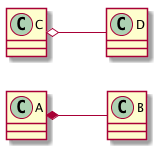
\includegraphics[height=6.5cm]{FAggregation.png}
\end{frame}

\begin{frame}[label=sec-1-10]{Aggregation}
\begin{itemize}
\item Aggregation
\begin{itemize}
\item ``Has-a''
\item Strong aggregation
\end{itemize}
\item Composition
\begin{itemize}
\item ``Consists-of''
\item weak aggregation
\end{itemize}
\end{itemize}

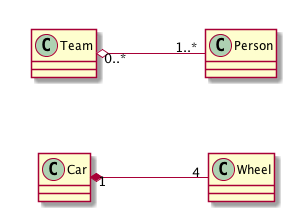
\includegraphics[height=4cm]{FAggregation2.png}
\end{frame}

\begin{frame}[label=sec-1-11]{Discussion: An Example}
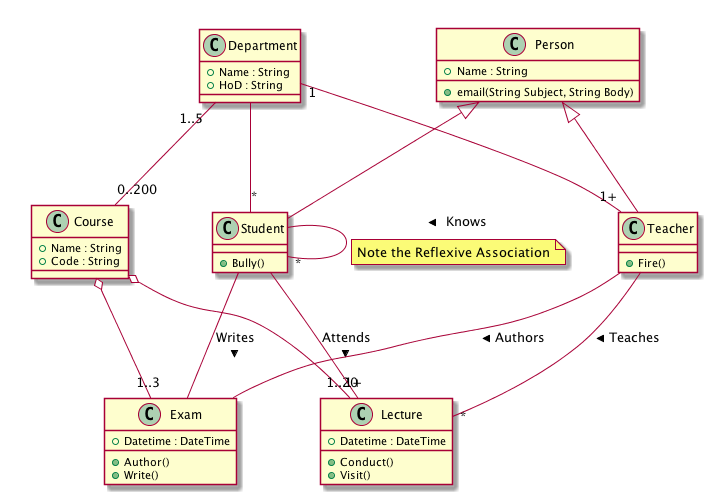
\includegraphics[height=6.5cm]{FExampleUniversity.png}
\end{frame}
\begin{frame}[label=sec-1-12]{Example}
\begin{itemize}
\item Conceptual Model for Discussion Forum Software
\end{itemize}
\end{frame}
\begin{frame}[label=sec-1-13]{Generalisation (Inheritance)}
Why
\begin{itemize}
\item Classification among concepts (is-a)
\item Code reuse, identifying commonalities
\end{itemize}

Example
\begin{itemize}
\item Vector Graphics Drawing Programme
\begin{itemize}
\item Point, Line, Arc, Polygon, Ellipse, Circle
\end{itemize}
\end{itemize}
\end{frame}
\begin{frame}[label=sec-1-14]{Generalisation: Hierarchy}
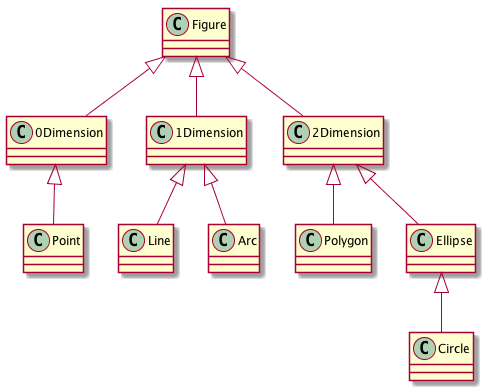
\includegraphics[height=6.5cm]{FInheritance.png}
\end{frame}

\begin{frame}[label=sec-1-15]{Generalisation: Hierarchy II}
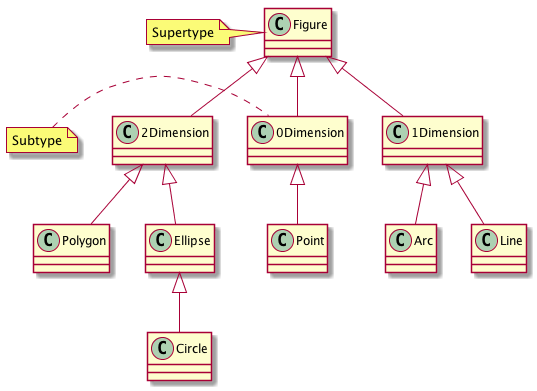
\includegraphics[height=6.5cm]{FInheritance2.png}
\end{frame}

\begin{frame}[label=sec-1-16]{Generalisation: Hierarchy III}
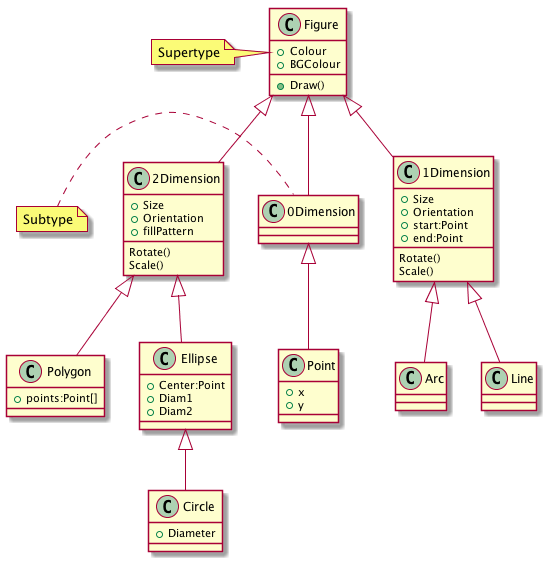
\includegraphics[height=6.5cm]{FInheritance3.png}
\end{frame}
\begin{frame}[label=sec-1-17]{Abstract Types}
\begin{itemize}
\item When no instances of the base class are desirable.
\item Example: There are no instances of the generic ``Figure'' base class.
\end{itemize}
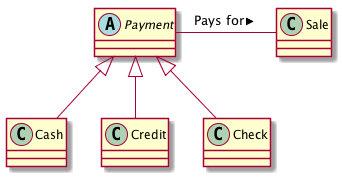
\includegraphics[height=4cm]{FInheritanceAbstract.png}
\end{frame}
\begin{frame}[label=sec-1-18]{Reflexive Associations}
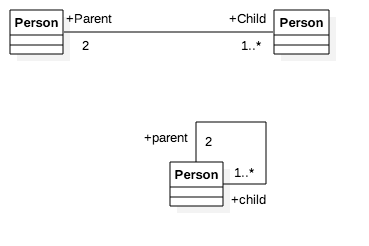
\includegraphics[width=.9\linewidth]{./IReflexive.png}
\end{frame}
\begin{frame}[label=sec-1-19]{Exotic UML: Association Attributes}
\only<1>{
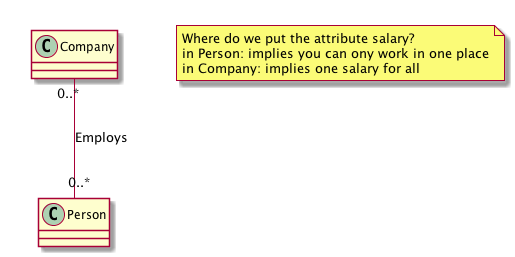
\includegraphics[height=6cm]{FAssociationAttributes0.png}
}

\only<2>{
One solution:

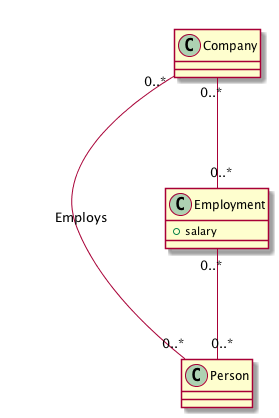
\includegraphics[height=6.5cm]{FAssociationAttributes1.png}
}

\only<3>{
Proper Solution:

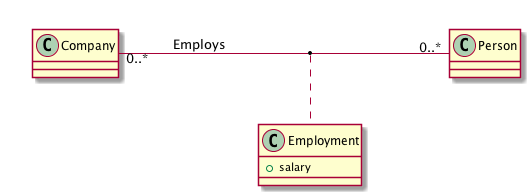
\includegraphics[width=10cm]{FAssociationAttributes2.png}
}
\end{frame}
% Emacs 25.1.1 (Org mode 8.2.10)
\end{document}